\chapter{列表、图片、链接}

\section{有序列表}

\subsection{有序列表(Ordered List)}

如果想在网页中展示有前后顺序的信息列表,如热度排行榜等,这类信息展示可以使用\lstinline|<ol>|-\lstinline|<li>|来实现有序列表。 \\

\begin{lstlisting}[style=htmlcssjs]
<ol>
    <li>信息</li>
    <li>信息</li>
</ol>
\end{lstlisting}

\begin{figure}[H]
    \centering
    
\includegraphics[scale=0.7]{img/C3/3-1/1.png}
    \caption{有序列表}
\end{figure}

\begin{lstlisting}[style=htmlcssjs, title=有序列表]
<!DOCTYPE html>
<html lang="en">
<head>
    <meta charset="UTF-8">
    <title>有序列表</title>
</head>
<body>
    <h3>2020年7月编程语言排行榜</h3>
    <ol>
        <li>C</li>
        <li>Java</li>
        <li>Python</li>
        <li>C++</li>
        <li>C#</li>
    </ol>
</body>
</html>
\end{lstlisting}

\subsection{序号类型}

\lstinline|<ol>|-\lstinline|<li>|在网页中显示的默认样式一般为每项\lstinline|<li>|前都自带一个序号,序号默认从1开始。通过修改\lstinline|<ol>|的type属性,也能对序号进行修改。 \\

\lstinline|<ol>|的type属性有5个值:

\begin{enumerate}
    \item 默认为数字序号:\lstinline|type="1"|
    \item 小写字母序号:\lstinline|type="a"|
    \item 大写字母序号:\lstinline|type="A"|
    \item 小写罗马数字序号:\lstinline|type="i"|
    \item 大写罗马数字序号:\lstinline|type="I"|
\end{enumerate}

\lstinline|<ol>|中设置start属性,可以指定开始序号。 \\

\lstinline|<ol>|中设置\lstinline|reversed="reversed"|属性,可以将列表序号降序排序。

\newpage

\section{无序列表}

\subsection{无序列表(Unordered List)}

网页上也有很多信息是无需按照先后次序排列的,如新闻列表、图片列表等,这类信息展示可以使用\lstinline|<ul>|-\lstinline|<li>|来实现无序列表。

\begin{lstlisting}[style=htmlcssjs]
<ul>
    <li>信息</li>
    <li>信息</li>
</ul>
\end{lstlisting}

\begin{figure}[H]
    \centering
    
\includegraphics[scale=0.8]{img/C3/3-2/1.png}
    \caption{无序列表}
\end{figure}

\lstinline|<ul>|-\lstinline|<li>|在网页中显示的默认样式一般为每项\lstinline|<li>|前都自带一个圆点。通过修改\lstinline|<ul>|的type属性,也能对前面的符号进行修改。 \\

\lstinline|<ul>|的type属性有2个值:

\begin{enumerate}
    \item 默认为实心小圆点:\lstinline|type="disc"|
    \item 实心正方形:\lstinline|type="square"|
\end{enumerate}

\begin{lstlisting}[style=htmlcssjs, title=无序列表]
<!DOCTYPE html>
<html lang="en">
<head>
    <meta charset="UTF-8">
    <title>无序列表</title>
</head>
<body>
    <h3>前端三剑客</h3>
    <ul>
        <li>HTML</li>
        <li>CSS</li>
        <li>JS</li>
    </ol>
</body>
</html>
\end{lstlisting}

淘宝网的导航栏就是利用\lstinline|<ul>|-\lstinline|<li>|的父子结构进行实现的。

\begin{figure}[H]
    \centering
    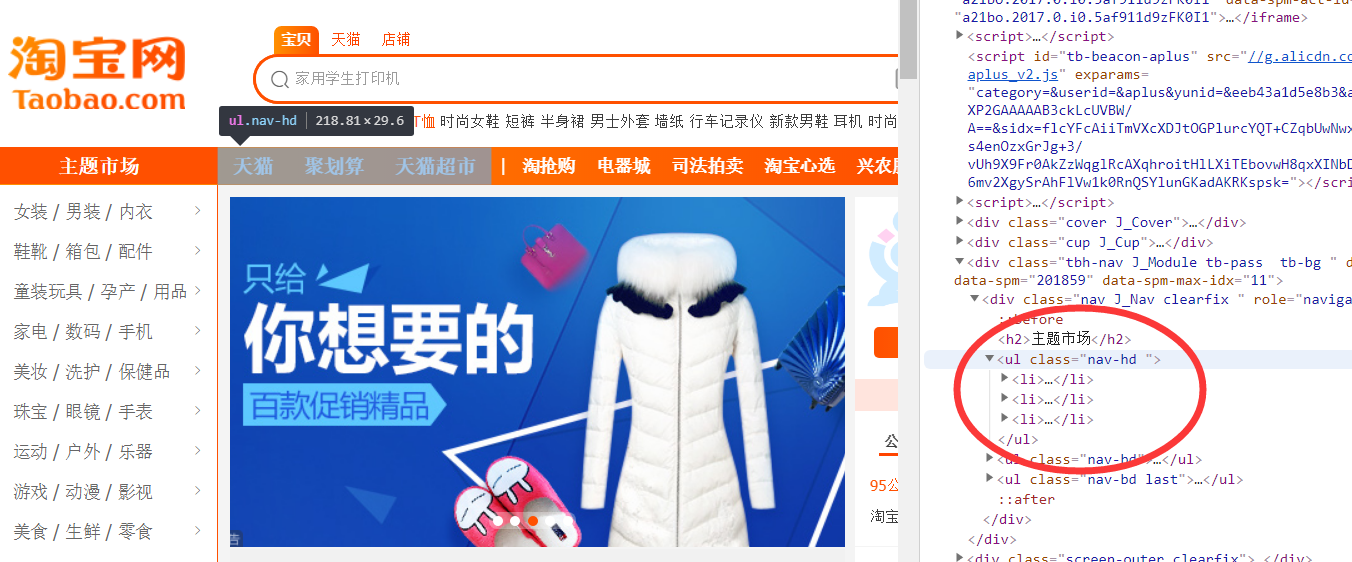
\includegraphics[scale=0.5]{img/C3/3-2/2.png}
    \caption{淘宝导航栏}
\end{figure}

\begin{lstlisting}[style=htmlcssjs, title=淘宝导航栏]
<!DOCTYPE html>
<html lang="en">
<head>
    <meta charset="UTF-8">
    <title>淘宝</title>
    <style type="text/css">
        ul {
            list-style: none;   /* 无序列表前面不带点 */
        }

        li {
            float: left;
            margin: 20px;
            padding: 5px;
            color: #000;
        }

        li:hover {
            background-color: #f40;     /* 淘宝红 */
            color: #fff;
            border-radius: 15px;
            cursor: pointer;
        }
    </style>
</head>
<body>
    <ul>
        <li>天猫</li>
        <li>聚划算</li>
        <li>天猫超市</li>
    </ul>
</body>
</html>
\end{lstlisting}

\newpage

\section{不发一张自拍吗?——img标签}

\subsection{img标签}

在网页的制作中为使网页炫丽美观,肯定是缺少不了图片,\lstinline|<img>|用于插入图片。 \\

\begin{lstlisting}[style=htmlcssjs]
<img src="图片地址" alt="下载失败时的替换文本" title="提示文本">
\end{lstlisting}

\begin{itemize}
    \item src属性用于标识图像的资源地址,资源地址可以来源于网上的URL,也可以来源于本地。

    \item alt属性指定图像的描述性文本,当图像下载不成功时,可看到该属性指定的文本。

    \item title属性提供当鼠标停留在图片时显示的文本。
\end{itemize}

\begin{lstlisting}[style=htmlcssjs, title=img标签, breaklines=true, breakatwhitespace=false]
<!DOCTYPE html>
<html lang="en">
<head>
    <meta charset="UTF-8">
    <title>img标签</title>
</head>
<body>
    <img src="https://ss0.bdstatic.com/70cFuHSh_Q1YnxGkpoWK1HF6hhy/it/u=3014023147,616635741&fm=26&gp=0.jpg" alt="皮卡丘.jpg" title="皮卡丘">
</body>
</html>
\end{lstlisting}

\newpage

\section{百度一下,你就知道——a标签}

\subsection{a标签}

使用\lstinline|<a>|可实现超链接,它在网页制作中可以说是无处不在,只要有链接的地方,就会有这个标签。 \\

\begin{lstlisting}[style=htmlcssjs]
<a href="目标网址" title="鼠标停留显示的文本">链接显示的文本</a>
\end{lstlisting}

\lstinline|<a>|中title属性提供的功能是当鼠标停留在链接文字时显示这个属性的文本内容,这个属性在实际网页开发中作用很大,主要方便搜索引擎了解链接地址的内容(语义化更友好)。

\begin{lstlisting}[style=htmlcssjs, title=a标签]
<!DOCTYPE html>
<html lang="en">
<head>
    <meta charset="UTF-8">
    <title>a标签</title>
</head>
<body>
    <a href="http://www.baidu.com" title="点击跳转百度">
        百度一下,你就知道
    </a>
</body>
</html>
\end{lstlisting}

只要为文本加入\lstinline|<a>|后,文字的颜色就会自动变为蓝色,被点击过的文本颜色会变为紫色,通过CSS样式可以对文字的颜色进行修改。 \\

\lstinline|<a>|中还有一个target属性,默认值为\_self,表示在同页面中打开被链接的文档。如果需要在新窗口打开被链接的文档,需要将target属性的值设置为\_blank。

\subsection{锚点(Anchor)}

\lstinline|<a>|最初的功能是记录锚点(记录位置),通过\lstinline|<a>|回到那个位置去。

\begin{lstlisting}[style=htmlcssjs, title=锚点, breaklines=true, breakatwhitespace=false]
<!DOCTYPE html>
<html lang="en">
<head>
    <meta charset="UTF-8">
    <title>锚点</title>
</head>
<body>
    <div id="div1" style="width: 100px; height: 100px; background-color: red;"></div>
    <div id="div2" style="width: 100px; height: 100px; background-color: blue;"></div>
    <br><br><br><br><br><br><br><br><br><br><br><br><br><br><br><br><br><br><br><br><br><br><br><br><br><br><br><br><br><br><br><br><br><br><br><br><br><br><br><br><br><br><br><br><br><br><br><br><br><br>
    <a href="#div1">跳转到div1</a>
    <a href="#div2">跳转到div2</a>
</body>
</html>
\end{lstlisting}

\lstinline|<a>|作为锚点的应用场景也很多,比如目录跳转。

\begin{figure}[H]
    \centering
    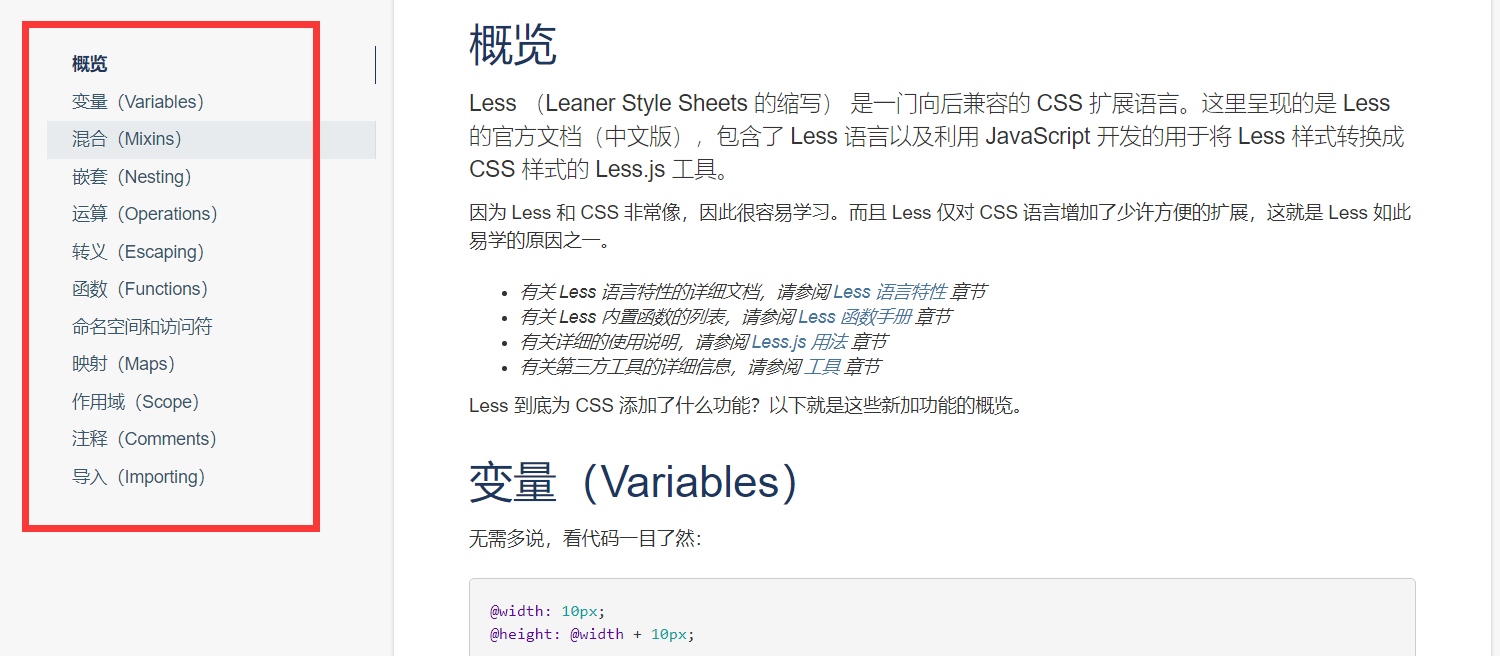
\includegraphics[scale=0.45]{img/C3/3-4/1.png}
    \caption{目录跳转}
\end{figure}

\subsection{协议限定符}

\lstinline|<a>|还能作为协议限定符,在点击链接时会强制执行JavaScript代码。

\begin{lstlisting}[style=htmlcssjs, title=协议限定符]
<!DOCTYPE html>
<html lang="en">
<head>
    <meta charset="UTF-8">
    <title>访问限定符</title>
</head>
<body>
    <a href="JavaScript: while(1) { alert('嘿嘿'); }">点我</a>
</body>
</html>
\end{lstlisting}

\newpage